%& --enable-write18
\RequirePackage{ifpdf}
\documentclass[a4paper,11pt]{article}
\usepackage{pgfplots,tocloft,textcomp,verbatim}
\pgfplotsset{width=7cm,compat=1.9}
%--This is to improve loading time
\usepgfplotslibrary{external}
\tikzexternalize
%--This is the end!
\renewcommand{\cftsecfont}{\normalfont}
\renewcommand{\cftsecpagefont}{\normalfont}
\renewcommand{\cftsecleader}{\cftdotfill{\cftsecdotsep}}
\renewcommand{\cftsecdotsep}{\cftdot}
\renewcommand{\cftsubsecdotsep}{\cftdot}
\renewcommand\cftsecaftersnum{.}
\renewcommand\thesection{\Roman{section}}
\author{Son To}
\date{June 13th, 2017}
\title{PGFPlot-A simple tutorial\footnote{This
tutorial is taken from
\href{https://www.sharelatex.com/learn/Pgfplots_package#/The_document_preamble}{this link}
with some modifications for personal pleasure!}}
\usepackage[pdftex,hyperindex=false,colorlinks,%
bookmarks,unicode]{hyperref}
\ifpdf
  \hypersetup{linkcolor=blue}
\else
  \hypersetup{linkcolor=black}
\fi
\begin{document}
  \maketitle
  \tableofcontents
  \clearpage
  \section{The Basic} \label{sec:1}
  Pgfplots is a powerful package specialized in creating
  powerful scientific \nolinebreak graphs.
  \begin{tikzpicture}
    \begin{axis}
      \addplot[color=blue]{exp(x)};
    \end{axis}
  \end{tikzpicture}
  % Here ends the first plot.
  \hskip 5pt
  % Here starts the 3d plot.
  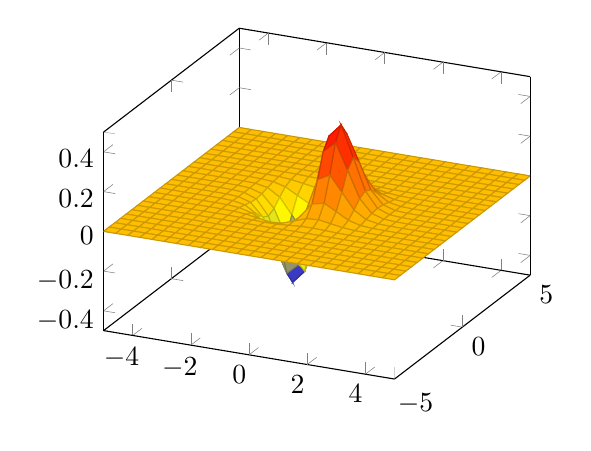
\begin{tikzpicture}
    \begin{axis}
      \addplot3[
      surf,
      ]{exp(-x^2-y^2)*x};
    \end{axis}
  \end{tikzpicture}
We now get to some more details on 2D plot.
\clearpage
\section{2D Plot}
What the heck...Let's do some damage!

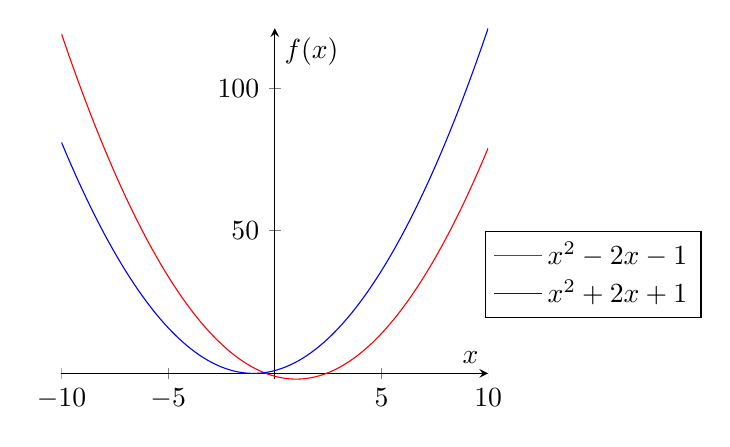
\begin{tikzpicture}
  \begin{axis}[
    axis lines= center,
    xlabel= $x$,
    ylabel= {$f(x)$},
    legend style={at={(axis cs:20,50)},anchor=north east},
    ]
    %We now add a red parabola
    \addplot[
    domain=-10:10,
    samples=100,
    color=red,
    ]
    {x^2-2*x-1};
    \addlegendentry{$x^2-2x-1$}
    %Now we add another parabola to the same axis
    \addplot[
    domain=-10:10,
    samples=100,
    color=blue
    ]
    {x^2+2*x+1};
    \addlegendentry{$x^2+2x+1$}
  \end{axis}
\end{tikzpicture}

Come on man!!!! Let's make some plots from data.
\clearpage
\subsection{Plotting from data}
I love to test \textcelsius

\begin{tikzpicture}
  \begin{axis}[
    title={Temperature dependence of CuSO$_4$\cdot5H$_2$O},
    xlabel={Temperature [\textcelsius]},
    ylabel={Solubility [g per 100g water]},
    xmin=0, xmax=100,
    ymin=0, ymax=120,
    xtick={0,20,...,100},
    ytick={0,20,...,120},
    legend pos=north west,
    ymajorgrids=true,
    grid style=dashed,
    ]

    \addplot[
      color=blue,
      mark=square,
    ]
    coordinates {
    (0,23.1)(10,27.5)(20,32)(30,37.8)(40,44.6)(60,61.8)%
    (80,83.8)(100,114)
    };
    \addlegendentry{CuSO$_4$\cdot5H$_2$0}
  \end{axis}
\end{tikzpicture}

When the data is in a file, put
\verb+\addplot table {file_with_the_data.dat}+
instead of using \verb+\addplot coordinates {}+.

\subsection{Scatter plots}
Scatter plot is used to represent information by using
some kind of marks, which are common, for example,
when computing statistical regression.

\begin{tikzpicture}
  \begin{axis}[
    enlargelimits=false,
    ]

    \addplot+[
    only marks,
    scatter,
    mark=halfcircle*,
    mark size=2.9pt,
    ]
    table[meta=ma]{data.dat};
  \end{axis}
\end{tikzpicture}

\subsection{Bar graphs}
Bar graphs are used to display gathered data.

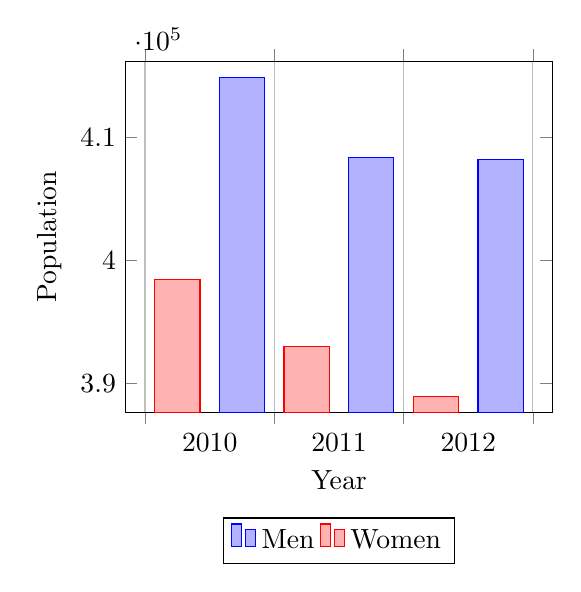
\begin{tikzpicture}
  \begin{axis}[
    x tick label style={
      /pgf/number format/1000 sep=},
    ylabel=Population,
    xlabel=Year,
    enlargelimits=0.05,
    legend style={at={(0.5,-0.3)},
    anchor=north, legend columns=2},
    ybar interval=0.7,
    ]

    \addplot
      coordinates {(2012,408184)(2011,408348)
      (2010,414870)(2009,412576)};
    \addplot
      coordinates {(2012,388950)(2011,393007)
      (2010,398449)(2009,395972)};
    \legend{Men,Women}
  \end{axis}
\end{tikzpicture}

\section{3D Plots}
For the basic plot, we refer to section~\ref{sec:1}. We now
use mesh feature for the plot.

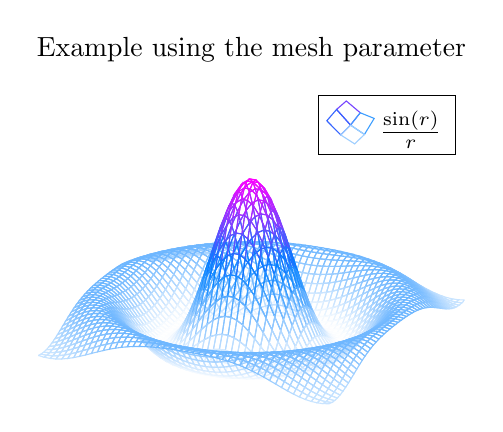
\begin{tikzpicture}
  \begin{axis}[
      title=Example using the mesh parameter,
      colormap/cool,
      hide axis,
    ]

    \addplot3[
    mesh,
    samples=50,
    domain=-8:8,
    ]
    {sin(deg(sqrt(x^2+y^2)))/sqrt(x^2+y^2)};
    \addlegendentry{$\frac{\sin(r)}{r}$}
  \end{axis}
\end{tikzpicture}

\subsection{Contour plot}
  The data needs to be calculated by external programs(%
  gnutplot, mathematica, etc\ldots)

  \begin{tikzpicture}
    \begin{axis}[
      title={Contour plot, view from top},
      view={0}{90},
      ]

      \addplot3[
        contour gnuplot={levels={0.8, 0.4, 0.2, -0.2}}
      ]
      {sin(deg(sqrt(x^2+y^2)))/sqrt(x^2+y^2)};
    \end{axis}
  \end{tikzpicture}
\end{document}
